
\begin{frame}{\citetitle{ArticuloDavidHidroponia_2022}$^*$ (1)}
\begin{columns}
\begin{column}{0.75\textwidth}
	\begin{itemize}  %del cuerpo académico Acuicultura Sustentable (UTMTB-CA-1)
        \item Los sistemas hidropónicos se basan en el cultivo de plantas sin la necesidad del suelo
        \item Las necesidades nutricionales de las plantas a cultivar son suministrandas a sus raíces mediante una solución nutritiva
		\item Se implementó un sistema hidropónico tipo DFT (Deep Flow Technique)
		\item Se trabaja en la incorporación de un monitoreo remoto para dicho sistema, con alarmas y notificaciones
	\end{itemize}
\end{column}
\begin{column}{0.25\textwidth}  
\includegraphics[width=0.98\textwidth]{2022_HidroponicosDavid/figs/dft}
\end{column}
%\begin{column}{0.25\textwidth}
%\includegraphics[width=0.98\textwidth]{2022_HidroponicosDavid/figs/iot}
%\end{column}
\end{columns} 
\footfullcite*{ArticuloDavidHidroponia_2022}
\end{frame}


\begin{frame}{\citetitle{ArticuloDavidHidroponia_2022} (2)}
\begin{columns}
\begin{column}{0.35\textwidth}
Componentes:
\begin{itemize}
        \item Raspberry Pi 3 B+ y módulo ESP32
        \item Sensores de temperatura, humedad, pH, conductividad eléctrica
        \item Bomba periférica de 1/2 HP y bombas peristálticas        
        \item Tubos de PVC
	\end{itemize}
\end{column}
\begin{column}{0.35\textwidth}  
\includegraphics[width=0.98\textwidth]{2022_HidroponicosDavid/figs/1}
\end{column}
\begin{column}{0.30\textwidth}  
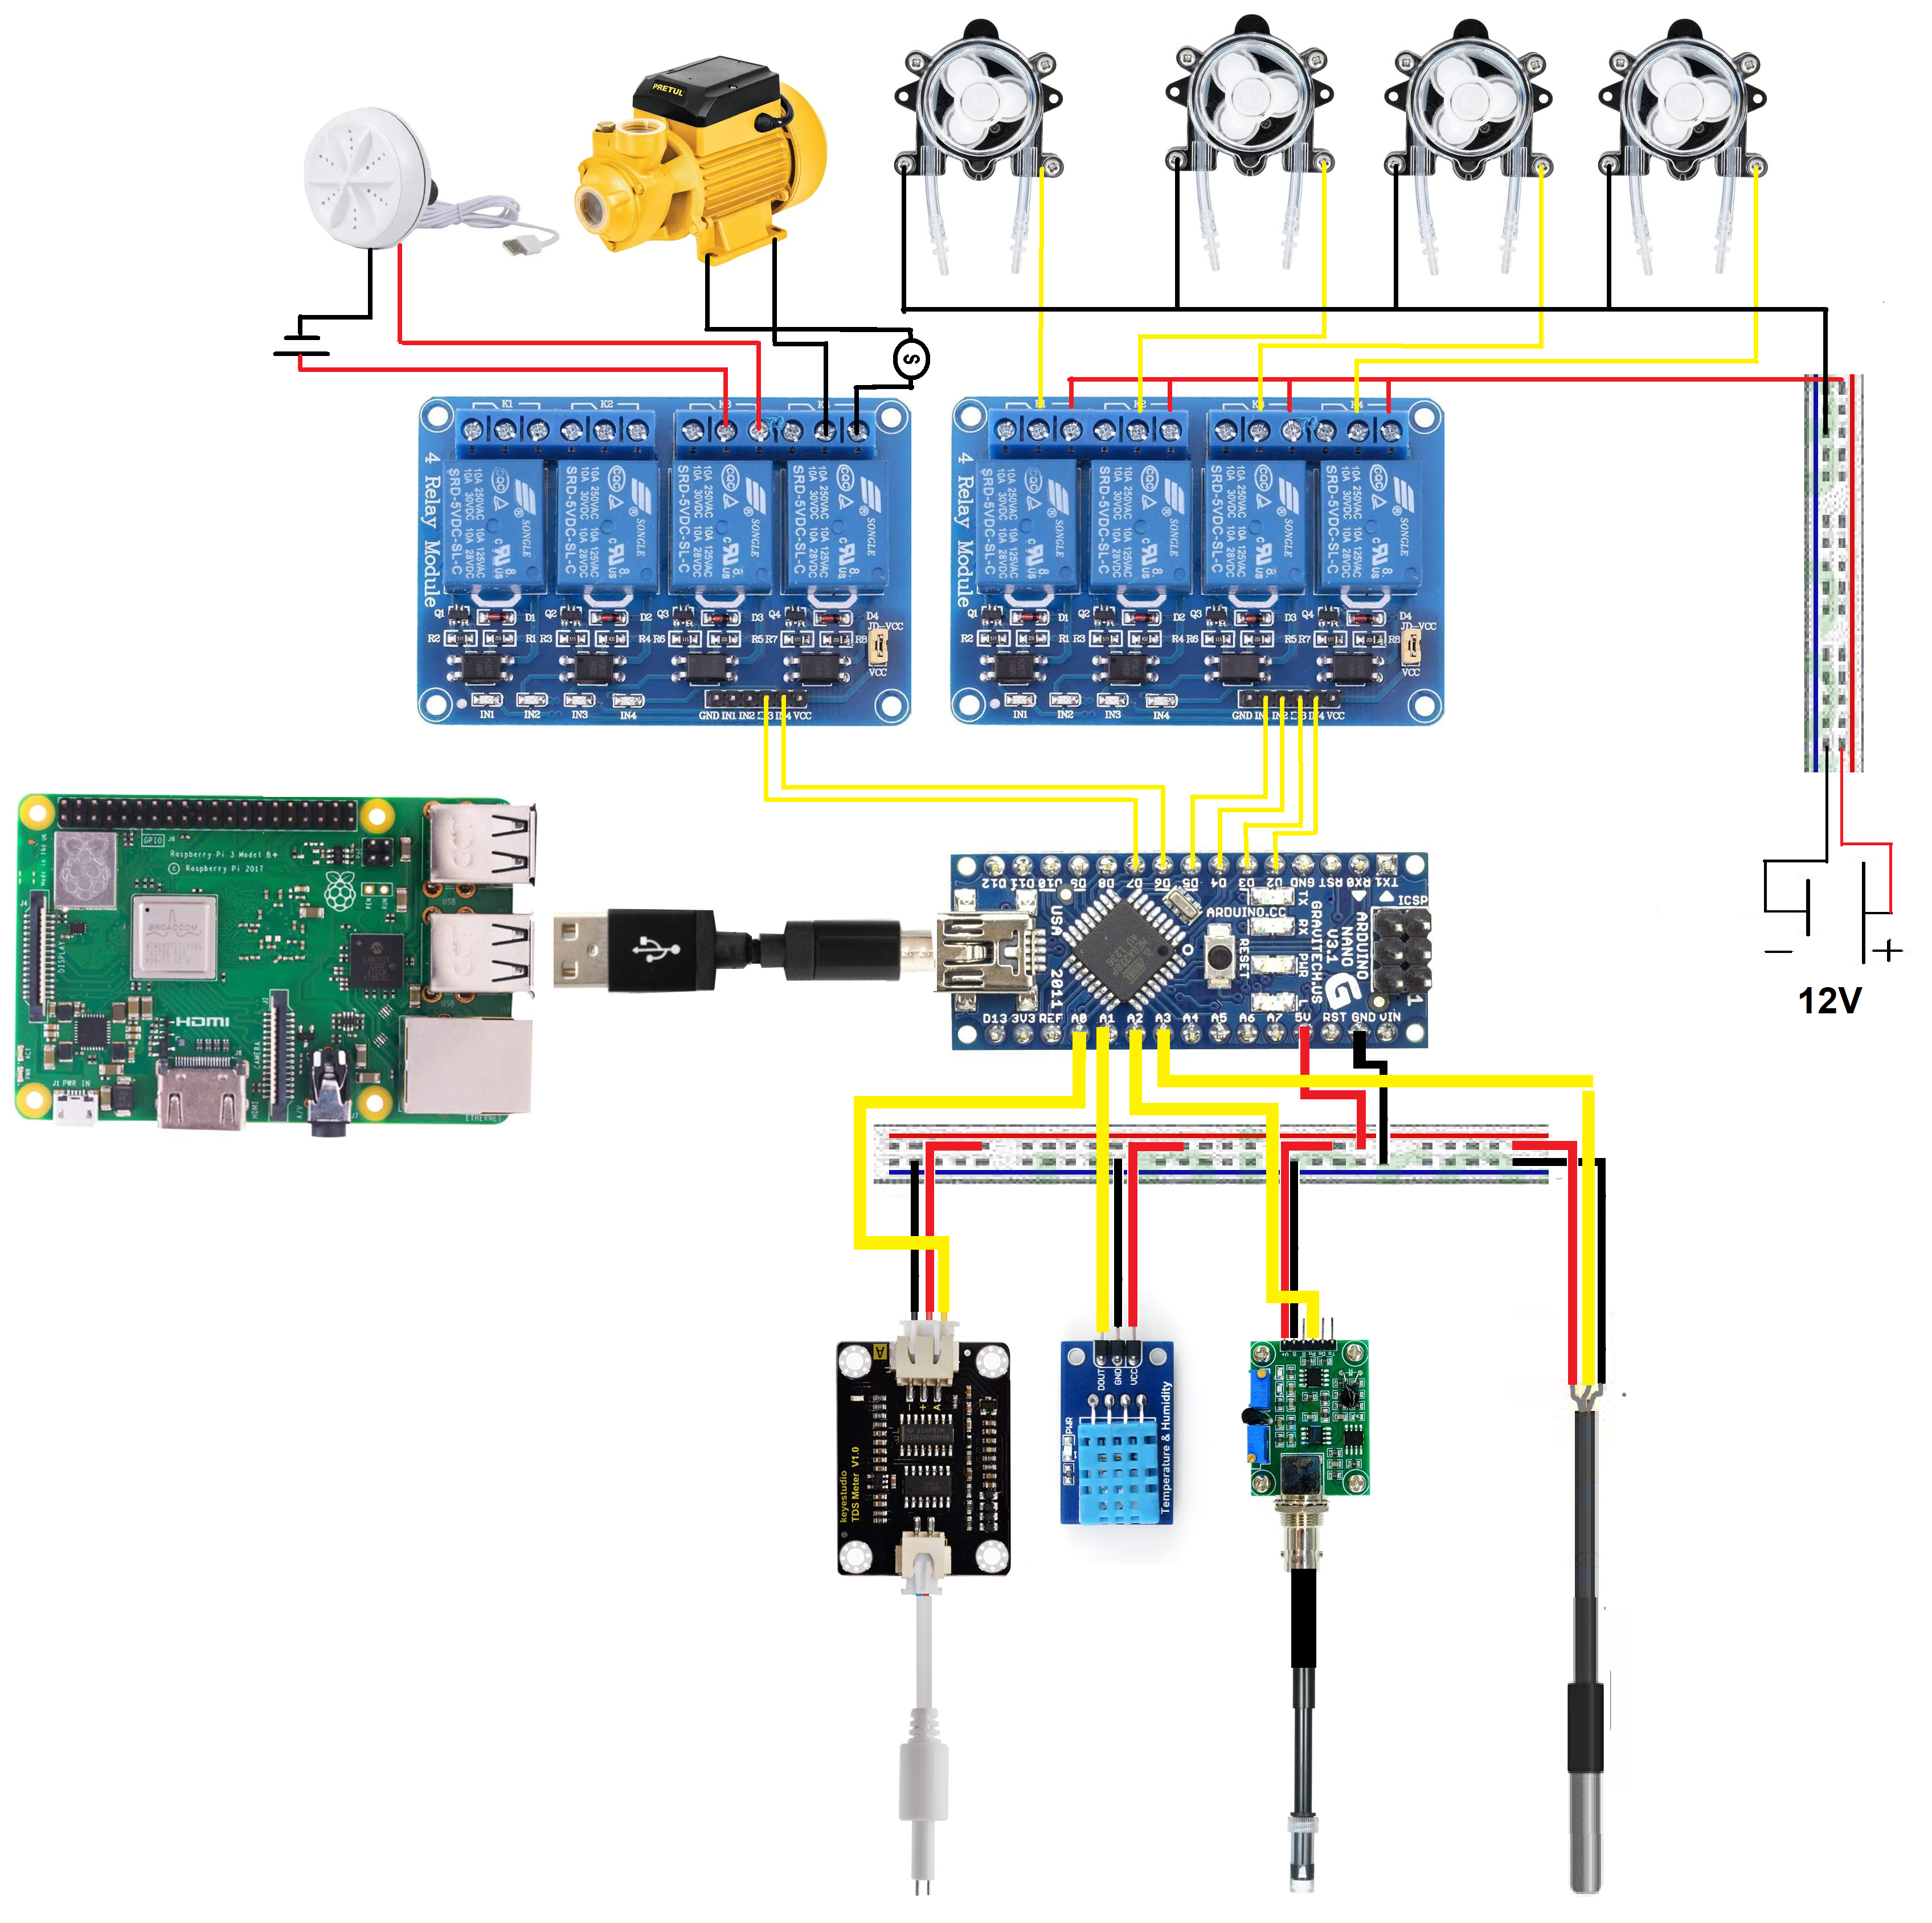
\includegraphics[width=0.98\textwidth]{2022_HidroponicosDavid/figs/Circuito_Articulo}
\end{column}
\end{columns} 
\end{frame}

\begin{frame}{\citetitle{ArticuloDavidHidroponia_2022} (3)}
\begin{columns}
\begin{column}{0.30\textwidth}
\begin{itemize}
		\item Se utiliza la plataforma Node-Red para visualizar las lecturas de los sensores
	\end{itemize}
\end{column}
\begin{column}{0.20\textwidth}  
         \includegraphics[width=0.98\textwidth]{2022_HidroponicosDavid/figs/app}

\end{column} 
\begin{column}{0.50\textwidth}  
         \includegraphics[width=0.98\textwidth]{2022_HidroponicosDavid/figs/servidor}
\end{column} 
\end{columns} 
\end{frame}






